\documentclass[12pt]{article}
\usepackage[utf8]{inputenc}
\usepackage[margin=1in]{geometry}
\usepackage[spanish]{babel}
\usepackage{parskip}
\usepackage{setspace}
\usepackage{amsmath, amssymb}
\usepackage{graphicx}
\usepackage{tikz}
%\usepackage{hyperref}

% Opciones de algunos paquetes.
\decimalpoint % {babel}: Pasar coma decimal de "coma" a "punto".
\onehalfspacing % {setspace}: Interlineado de 1.5.
\graphicspath{{./img/}} % {graphicx}: Ruta (path) donde se encuentran las imagenes.
\usetikzlibrary{babel} % {tikz}: Para que tikz no conflictue con {babel} con figuras como "->".
\usetikzlibrary{arrows.meta} %{tikz}: Librería para personalizar las cabezas de las flechas.


% Encabezado.
\title{Clase 5. Ecuaciones Paramétricas para Líneas y Curvas.}
\author{MIT 18.02: Multivariable Calculus.}
\date{}


\begin{document}

\maketitle

\begin{abstract}
\noindent Una línea y una curva no solo pueden ser representadas por medio de una función o ecuación de dos variables $x$ e $y$, donde $y = f(x)$ o $x = g(y)$. También es posible definir a ambas en términos de una \textbf{tercera variable} $t$, tal que $x(t)$ e $y(t)$. El término $t$ se conoce como \textbf{parámetro} y, por este motivo, $x(t)$ e $y(t)$ reciben el nombre de \textbf{ecuaciones paramétricas}, las cuales estudiaremos a continuación.
\end{abstract}


\section{Ecuaciones Paramétricas de una Línea.}

Supongamos que queremos conocer una línea en el espacio (i.e, en $\mathbb{R}^{3}$). Una manera de lograrlo sería buscar dos ecuaciones de planos que se intersecten. Para ello, resolvemos un sistema con éstas ya que con sus soluciones seremos capaces de formar una recta. El problema es que corresponderán a infinitos puntos (al menos más de uno).

Una forma más expedita de encontrar una recta en el espacio sería tomar \textbf{un solo punto}, pero que esté \textbf{en movimiento por una unidad de tiempo} y lo haga de forma lineal, puesto que la figura que se forma con su \textbf{trayectoria}\footnote{Es decir,  el ``camino'' que va dejando.} será una línea. En ese sentido, su coordenada estará en \textbf{función de una variable adicional} $t$ y será de la forma $(x(t), \ y(t), \ z(t))$.

Cuando una figura está representada por un punto cuyas coordenadas están definidas en términos de una nueva variable $t$ conocida como \textbf{parámetro}, las funciones adentro de la terna ordenada\footnote{También se aplica para puntos en dos, una o infinitas dimensiones.} $(f(t), \ g(t), \ h(t))$ reciben el nombre de \textbf{Ecuaciones Paramétricas}.

Por lo tanto, las ecuaciones de $(x(t), \ y(t), \ z(t))$ que forman la trayectoria lineal que vimos anteriormente corresponden a las \textbf{Ecuaciones Paramétricas de una Línea}.

\newpage

\textbf{Ejemplo 1.} Suponga que una partícula se mueve a través de una línea que pasa por los puntos $Q_{0} = (-1, \ 2, \ 2)$ y $Q_{1} = (1, \ 3, \ -1)$ a una rapidez constante y en un tiempo $t$, donde en $t = 0$ está en $Q_{0}$. Calcule en qué ubicación se encuentra en un tiempo $t$.

\textbf{Solución.} Lo primero que podemos considerar, es que la ubicación de la partícula está en términos de $t$. Por lo tanto, podemos definir su posición como $Q(t) = (x(t), \ y(t), \ z(t))$.

En segundo lugar, la rapidez con que se mueve la partícula es constante y lo hace de forma lineal, de manera que como comienza en $Q_{0}$ en $t = 0$, podemos asumir que en $t = 1$ estará en $Q_{1}$ ya que, además, ambos puntos son colineales.

Como la partícula se moverá al menos desde $Q_{0}$ hasta $Q_{1}$ y su posición estará en función de $t$, podemos conocer a esta última a partir de vectores a través de la siguiente igualdad:
\begin{align*}
  \overrightarrow{Q_{0}Q(t)} &= t \cdot \overrightarrow{Q_{0}Q_{1}} \\
  \langle x(t) - (-1), \ y(t) - 2, \ z(t) - 2 \rangle &= t \cdot \langle 1 - (-1), \ 3 - 2, \ - 1 - 2 \rangle \\
  \langle x(t) + 1, \ y(t) - 2, \ z(t) - 2 \rangle &= \langle 2t, \ t, \ -3t \rangle
\end{align*}
En la Clase 1 señalamos que dos o más vectores son iguales si sus componentes y dirección también lo son. Sabemos que $Q(t)$ se está moviendo desde $Q_{0}$ hasta (o a través de) $Q_{1}$ y hemos asumido que $\overrightarrow{Q_{0}Q_{1}}$ está en la misma dirección. Por lo tanto, para que se cumpla la ecuación de arriba tenemos que igualar sus componentes.
\begin{align*}
2t &= x(t) + 1 & t &= y(t) - 2 & -3t &= z(t) - 2 \\
x(t) &= 2t - 1 & y(t) &= t + 2 & z(t) &= -3t + 2
\end{align*}
Por consiguiente, las coordenadas de la posición de la partícula para cada tiempo $t$ estarán dadas por las siguientes ecuaciones paramétricas:
\[
  Q(t) = (2t - 1, \ t + 2, \ -3t + 2)
\]
\textbf{Ejemplo 2.} Evalúe si el plano $x + 2y + 4z = 7$ es intersectado por la línea que pasa por los puntos $Q_{0} = (-1, \ 2, \ 2)$ y $Q_{1} = (1, \ 3, \ -1)$. De ser así, señale en qué lugar se cruzan.

\textbf{Solución.} Primero debemos saber cuál es la recta que intersecta o no al plano señalado en el ejemplo. Para ello, podemos parametrizar un punto $Q(t)$ a partir de $Q_{0}$ y $Q_{1}$.

Las ecuaciones paramétricas de $Q(t)$ por medio de $Q_{0}$ y $Q_{1}$ las conocimos en el ejemplo anterior, donde:
\[
  Q(t) = (2t - 1, \ t + 2, \ -3t + 2)
\]
Para saber si la línea que se forma a partir de $Q(t)$ intersecta o no al plano, debemos reemplazar sus incógnitas $x$, $y$ y $z$ con las ecuaciones paramétricas del punto mencionado. Ante esto, tenemos tres posibilidades que se resumen en la siguiente tabla:

\begin{table}[hbt!]
\centering

\begin{tabular}{c c c c}
\hline
$t$ & Igualdad & Comportamiento de Línea & Intersección: Cantidad de puntos \\
\hline
Existe & - & Intersecta al plano & Uno \\
No existe & Se cumple & Pertenece al plano & Todos los de la línea \\
No existe & No se cumple & Paralela al plano & Ninguno \\
\hline
\end{tabular}

\end{table}

Como vemos en la tabla de arriba, una posibilidad es que al reemplazar a las incógnitas de la ecuación del plano con las coordenadas de $Q(t)$, obtengamos un valor para el $t$, lo que quiere decir que la línea se intersecta con esta figura y el punto podemos conocerlo al reemplazar el valor del parámetro en éste.

No obstante, también es posible que el parámetro se cancele al realizar el álgebra para conocerlo. Ahí se presentan dos opciones: Que encontremos una constante que sea igual a la que está en el lado derecho de la ecuación y que corresponde al valor donde se intersecta esta figura con el eje $z$, o que sean números distintos. En el primer caso, significa que la recta está en el plano, mientras que el segundo que no lo está ya que es paralela a éste.

Por lo tanto, reemplacemos a $x$, $y$ y $z$ de la ecuación del plano con las coordenadas de $Q(t)$ para conocer a $t$, en caso de existir.
\begin{align*}
  (2t - 1) + 2(t + 2) + 4(-3t + 2) &= 7 \\
         2t - 1 + 2t + 4 - 12t + 8 &= 7 \\
                                 t &= \frac{1}{2}
\end{align*}
Como encontramos un valor para $t$, entonces podemos dar por asegurado que la recta formada por las ecuaciones paramétricas de $Q(t)$ intersecta al plano $x + 2y + 4z = 7$. Reemplcemos al parametro en el punto para saber dónde en particular ocurre este cruce.
\[
  Q\left(\frac{1}{2}\right) = \left(2\left(\frac{1}{2}\right) - 1, \ \left(\frac{1}{2}\right) + 2, \ -3\left(\frac{1}{2}\right) + 2\right)
                            = \left(0, \ \frac{5}{2}, \ \frac{1}{2}\right)
\]
Así, podemos concluir que la recta formada por $Q(t) = (2t - 1, \ t + 2, \ -3t + 2)$ intersecta al plano $x + 2y + 4z = 7$ en el punto $(0, \ 5/2, \ 1/2)$.


\section{Ecuaciones Paramétricas de una Curva.}

En la sección anterior usamos ecuaciones paramétricas para representar a una línea, pero éstas pueden ser utilizadas para cualquier tipo de curva generada por un movimiento arbitrario, sea en un plano o en el espacio. Un ejemplo de aquello es la \textbf{cicloide}.

Si bien existen distintos tipos de cicloides\footnote{También es posible generar una cicloide a partir del movimiento de un péndulo.}, la que veremos en esta clase es una curva que se forma a partir de la trayectoria dejada por un punto ubicado en la circunferencia de un círculo que rueda sobre una recta horizontal.

A continuación tenemos una ciloide, donde $P$ es el punto en movimiento y cuya trayectoria la genera.

\begin{figure}[hbt!]
\centering
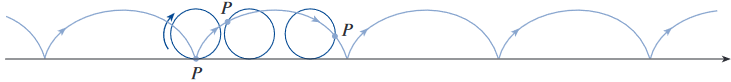
\includegraphics[scale=0.7]{cycloid.png}
\caption{Stewart, J (2017). \textit{Cálculo. Trascendentes Tempranas}. Pp. 643.}
\end{figure}

Por lo tanto, para trazar la cicloide tenemos que conocer la \textbf{posición del punto} mientras rueda el círculo, la cual solo es posible de obtener por medio de \textbf{ecuaciones paramétricas}.

Digamos que tenemos un círculo de radio $r = a$ con centro $B$ y un punto $P$ en su circunferencia, el cual está rodando a una rapidez constante a lo largo del eje $x$ del plano cartesiano\footnote{Si fuese un camino, sería uno sin irregularidades o totalmente plano.}, donde $A$ es el punto donde toca dicho lugar.

\begin{figure}[hbt!]
\centering

\begin{tikzpicture}
% Celdas de ayuda.
%\draw[help lines] (-7, -3) grid (7, 3);

% Ejes.
\draw [-{Stealth[length=3mm, width=2mm]}] (-4.5, -2) -- (5, -2) node [below]{$x$};
\draw [-{Stealth[length=3mm, width=2mm]}] (-4.5, -2) -- (-4.5, 2) node [left]{$y$};

% Radio circulo.
\draw (-2, -2) -- (-2, -0.5);
\node at (-2, -1.25) [right] {$a$};

% Linea con que se forma el angulo \theta.
\draw [dashed] (-2, -0.5) -- (-3.48, -0.7);
\node at (-2.5, -1) {$\theta$};

% Circulo (con el centro marcado con una X).
\draw (-2, -0.5) circle (1.5cm); % la coordenada (-2, -0.5) es el centro del circulo.
\draw [fill=black] (-2, -0.5) node [above]{$B$} circle (0.8mm);
\draw [fill=black] (-2, -2) node [below]{$A$} circle (0.8mm);

% Punto P.
\draw [fill=black] (-3.48, -0.7) circle (0.8mm);
\node at (-3.7, -0.4) {$P$};

% Origen.
\node at (-4.7, -1.8) {$0$};

% Efecto de movimiento del circulo.
\draw [->, line width=0.3mm] (-2.5, 1.2) arc (125:75:1cm);

\end{tikzpicture}

\end{figure}

Para conocer las ecuaciones paramétricas de $P$, necesitamos definir el parámetro de su coordenada. En este caso usaremos el ángulo $\theta$ en radianes que se forma entre los radios $\overline{AB}$ y $\overline{PB}$, puesto que es la variable que nos indica mejor la posición de este punto mientras rueda el círculo.
\[
  P = (x(\theta), \ y(\theta))
\]

El medio que usaremos para obtener las ecuaciones $x(\theta)$ e $y(\theta)$, serán los componentes del vector $\overrightarrow{OP}$ que podemos conocer a partir de la suma entre los vectores $\overrightarrow{OA}$, $\overrightarrow{AB}$ y $\overrightarrow{BP}$, con $O$ siendo el origen, los cuales son más sencillos de conocer.
\[
  \overrightarrow{OP} = \overrightarrow{OA} + \overrightarrow{AB} + \overrightarrow{BP}
\]
Geométricamente, nos estamos refiriendo a lo siguiente:

\begin{figure}[hbt!]
\centering

\begin{tikzpicture}
% Celdas de ayuda.
%\draw[help lines] (-7, -3) grid (7, 3);

% Ejes.
\draw [-{Stealth[length=3mm, width=2mm]}] (-4.5, -2) -- (5, -2) node [below]{$x$};
\draw [-{Stealth[length=3mm, width=2mm]}] (-4.5, -2) -- (-4.5, 2) node [left]{$y$};

% Radio circulo.
\node at (-2, -1.25) [right] {$a$};

% Linea con que se forma el angulo \theta.
\node at (-2.5, -1) {$\theta$};

% Circulo (con el centro marcado con una X).
\draw (-2, -0.5) circle (1.5cm); % la coordenada (-2, -0.5) es el centro del circulo.
\draw [fill=black] (-2, -0.5) node [above]{$B$} circle (0.8mm);
\draw [fill=black] (-2, -2) node [below]{$A$} circle (0.8mm);

% Punto P.
\draw [fill=black] (-3.48, -0.7) circle (0.8mm);
\node at (-3.7, -0.4) {$P$};

% Origen.
\node at (-4.7, -1.8) {$0$};

% Efecto de movimiento del circulo.
\draw [->, line width=0.3mm] (-2.5, 1.2) arc (125:75:1cm);

% Vectores
\draw [->, cyan, line width=0.5mm] (-4.5, -2) -- (-2, -2); % OA
\draw [->, cyan, line width=0.5mm] (-2, -2) -- (-2, -0.5); % AB
\draw [->, cyan, line width=0.5mm] (-2, -0.5) -- (-3.48, -0.7); % BP
\draw [->, red, line width=0.5mm] (-4.5, -2) -- (-3.48, -0.7); % OP

% Punto O.
\node at (-4.5, -2.25) {$O$};

\end{tikzpicture}

\end{figure}

Comencemos buscando los componentes de $\overrightarrow{OA}$. Recordemos que $A$ es el punto que está tocando al eje $x$ mientras el círculo rueda a una rapidez constante. Si asumimos que estuvo en el origen $O(0, \ 0)$, entonces la distancia $d(OA)$ que es equivalente a $|\overrightarrow{OA}|$ será igual a la longitud del arco\footnote{La longitud del arco de un círculo corresponde al producto entre la fracción del ángulo que está subtendido del arco con respecto al ángulo del círculo completo (ambos en radianes) y la circunferencia de este último.\[\overline{AP} = \frac{\theta}{2 \pi} \cdot (2 \pi a) = a \cdot \theta\]} $\overline{AP}$.
\[
  \overline{AP} = d(OA) = |\overrightarrow{OA}| = a \cdot \theta
\]
Y como $\overrightarrow{OA}$ está horizontalmente en el eje $x$, entonces sus componentes son:
\[
  \overrightarrow{OA} = \langle a \theta, \ 0 \rangle
\]
En cuanto a $\overrightarrow{AB}$, como es paralelo a $y$ y su magnitud es igual al radio del círculo, podemos garantizar que sus componentes son:
\[
  \overrightarrow{AB} = \langle 0, \ a \rangle
\]

Con respecto a $\overrightarrow{BP}$, primero veamos que su magnitud es igual al radio del círculo, ya que comprende entre el centro $B$ y el punto $P$ que está en su circunferencia.
\[
  \left|\overrightarrow{BP}\right| = a
\]
Además, entre $\overrightarrow{BP}$ y parte de $\overrightarrow{AB}$, junto con $\theta$, podemos formar un triángulo rectángulo.

\begin{figure}[hbt!]
\centering

\begin{tikzpicture}
%\draw [help lines] (-3, -3) grid (3, 3);

% Letra de los puntos.
\node at (1.2, 2.5) {$B$};
\node at (-2.4, 0.7) {$P$};
\node at (1.3, -1.5) {$A$};

% Puntos.
\draw [fill=black] (-2, 0.5) circle (0.8mm); % Punto P
\draw [fill=black] (1, 2.2) circle (0.8mm); % Punto B (centro del circulo)
\draw [fill=black] (1, -1.5) circle (0.8mm); % Punto A

\draw (-2, 0.5) -- (1, 0.5);
\draw [->, cyan, line width=0.5mm] (1, 2.2) -- (-2, 0.5); % Vector BP
\draw [->, cyan, line width=0.5mm] (1, -1.5) -- (1, 2.2); % Vector AB

% radio a.
\node at (-0.5, 1.6) {$a$};

\draw [dashed] (-3, 2.2) -- (3, 2.2);
\draw [dashed] (-2, 0.5) -- (-2, 2.2);
\draw [dashed] (1, 2.2) -- (1, 3);


% Angulos.
\node at (0.8, 1.8) {$\theta$};
\draw (1, 1) -- (0.5, 1) -- (0.5, 0.5);
\end{tikzpicture}

\end{figure}

Como podemos observar, a partir de los catetos del triángulo rectángulo de arriba podemos conocer los componentes de $\overrightarrow{BP}$ por medio de las funciones trigonométricas $\sin(\theta)$ y $\cos(\theta)$.
\begin{align*}
  \sin(\theta) &= \frac{\mathrm{OP}}{a} & \cos(\theta) &= \frac{\mathrm{ADY}}{a} \\
  a \cdot \sin(\theta) &= \mathrm{OP} & a \cdot \cos(\theta) &= \mathrm{ADY}
\end{align*}
Ahora bien, veamos que el ángulo $\theta$ está en el tercer cuadrante del plano cartesiano que se forma a partir del centro $B$ del círculo, por lo que los valores de OP y ADY serán negativos debido a que el $\sin(\theta) < 0$ y $\cos(\theta) < 0$ en dicho lugar. Por lo tanto:
\[
  \overrightarrow{BP} = \langle -a \cdot \sin(\theta), \ -a \cdot \cos(\theta) \rangle
\]
Por consiguiente, los componentes de $\overrightarrow{OP}$ son:
\begin{align*}
  \overrightarrow{OP} &= \langle a \theta, \ 0 \rangle + \langle 0, \ a \rangle + \langle -a \cdot \sin(\theta), \ -a \cdot \cos(\theta) \rangle \\
                      &= \langle a \theta - a \sin(\theta), \ a - a \cos(\theta) \rangle
\end{align*}
y las ecuaciones paramétricas de $P$ con las cuales obtenemos la cicloide, son:
\[
  P = (a \theta - a \sin(\theta), \ a - a \cos(\theta))
\]
donde $\theta$ es el parámetro (varía) y $a$ el radio del círculo (se mantiene constante).

\end{document}
